\section{Webcam}

%% ###################################################################################################
%%   Unterkapitel                                                                                                                                                                              #
%% ###################################################################################################

\subsection{Warteschlange}
Die Warteschlange sollte verhindern, dass mehrere Benutzer gleichzeitig die Webcam bedienen. Jeder der die Webcam bedienen möchte soll sich in einer Warteschlange registrieren. Ist diese erfolgt und der Benutzer an der Reihe, hat er 20 Sekunden Zeit die Webcam zu bedienen. Die Registrierung soll über einen Button Registrieren erfolgen.

\subsubsection{Funktionsweise Warteschlange}
Die Warteschlange funktioniert folgendermassen, registriert sich ein Benutzer per Klick auf den Registrierungsbutton wird eine Sessionid gelöst. Anschliessend wird in der Datenbank abgefragt ob weitere Benutzer in der Warteschlange sind. Hierbei bestehen zwei Möglichkeiten:\\

Keine weiteren Benutzer:\\
Die Session ID mit dem Zeitstempel und der Wartezeit für den nächsten wird in die Datenbank geschrieben. Dies ist in Bild \ref{img:tblqueue} zu sehen. 
\begin{figure}[h!]
  \fbox{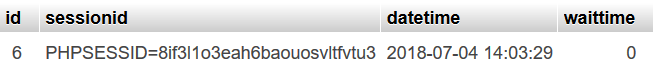
\includegraphics[width=\textwidth-2\fboxsep-2\fboxrule]{img/tblqueue.png}}
	\centering
	%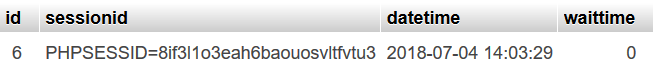
\includegraphics[width=1\linewidth]{img/tblqueue}
	\caption{Datenbankeintrag, wenn keine weiteren Benutzer da sind}
	\label{img:tblqueue}
\end{figure}

Vorgehen mehrere Benutzer:\\

Sind mehrere Benutzer in der Warteschlange wird die Wartezeit in Sekunden angezeigt
\begin{figure}[h!]
  \fbox{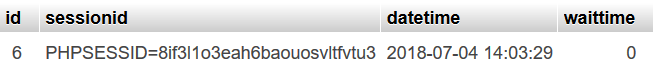
\includegraphics[width=\textwidth-2\fboxsep-2\fboxrule]{img/tblqueue.png}}
	\centering
	%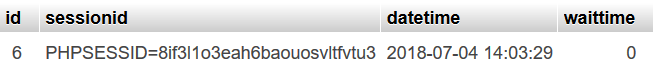
\includegraphics[width=1\linewidth]{img/tblqueue}
	\caption{Datenbankeintrag, wenn keine weiteren Benutzer da sind}
	\label{img:tblqueue}
\end{figure}
%% ###################################################################################################
%%   Unterkapitel                                                                                                                                                                              #
%% ###################################################################################################

\subsection{Selektive Zoombeschränkung}


%% ###################################################################################################
%%   Unterkapitel                                                                                                                                                                              #
%% ###################################################################################################

\subsection{Foto-Funktion}
